\documentclass[a4paper, 10pt, openany]{book} % openany - глава с новой страницы
\usepackage[russian]{babel} % добавление русского языка
\usepackage{amsfonts} % обозначение множеств
\usepackage{amsmath} % жирный шрифт в формулах
\pagestyle{myheadings}
\special{papersize=170mm,240mm}
\textheight 187mm % 200-(12+25)*0.35146 = 186.99598
\textwidth 130mm % максимальная ширина строчки 
\headheight13.6pt % = 0.48 mm
\oddsidemargin -5.4mm % левое поле (с учетом одного дюйма)
\topmargin -5.4mm % верхнее поле (с учетом одного дюйма)
\usepackage{setspace}
\singlespacing

\usepackage{listings}
\usepackage{graphicx}
\usepackage{subcaption}
\usepackage[%  
colorlinks=true,
pdfborder={0 0 0},
linkcolor=red
]{hyperref}

% Работа с колонтитулами
\usepackage{fancybox,fancyhdr}
\pagestyle{fancy}
\fancyhead{}
\fancyhead[LE,RO]{\thepage}
\fancyhead[RE, LO]{Учебник по машинному обучению} 
\fancyfoot{}

% настройки абзацев
\usepackage{indentfirst}
\setlength{\parindent}{5ex}
\setlength{\parskip}{1em}

\begin{document}
	
	\tableofcontents % оглавление
	
	\newpage
	
	\chapter{Введение}
	
	\section{Машинное обучение}
	
	\textbf{Машинное обучение} -- это наука, изучающая алгоритмы, автоматически улучшающиеся благодаря опыту.
	
	Большинство решений задач можно представить в виде функции:
	\begin{equation*}
		\textit{Примеры (samples)} \rightarrow \textit{Предсказания (targets)}.
	\end{equation*}
	Данная функция -- \textbf{модель}, а набор примеров -- \textbf{обучающая выборка (dataset)}.
	\begin{equation*}
		\text{Обучающая выборка} = \text{Объекты} + \text{Ответы}.
	\end{equation*}
	Качество таких предсказаний измеряют \textbf{метриками} -- функциями, которые показывают насколько полученные предсказания похожи на правильные ответы. Примером метрики является \textbf{среднее абсолютное отклонение}:
	\begin{equation*}
		MAE(f,X,y) = L(f,X,y) = \frac{1}{N}\sum_{i=1}^{N}|f(x_i) - y_i|. 
	\end{equation*}
	На сегодня достаточно знать два типа моделей -- \textbf{градиентный бустинг на решающий деревьях} и \textbf{нейросетевые модели}.
	
	Метрику, которую используют при поиске оптимальной модели -- \textbf{функция потерь, лосс-функцией (loss)}.
	
	\section{Виды задач}
	
	Определенные выше задачи -- \textbf{обучение с учителем(supervised learning)}, так как правильные ответы были даны заранее. Виды таких обучений: 
	\begin{itemize}
		\item $\mathbb{Y} = \mathbb{R}$ или $\mathbb{Y} = \mathbb{R}^M$ -- \textbf{регрессия};
		\item $\mathbb{Y} = \{0,1\}$ -- \textbf{бинарная классификация};
		\item $\mathbb{Y} = \{1,..,K\}$ -- \textbf{многоклассовая (multiclass) классификация};
		\item $\mathbb{Y} = \{0,1\}^K$ -- \textbf{многоклассовая классификация с пересекающимися классами (multilabel classification)};
		\item $\mathbb{Y}$ -- конечное упорядоченное множество -- \textbf{ранжирование}.
	\end{itemize}
	
	Имеется другой класс задач--\textbf{обучение без учителя (unsupervised learning)}-- для которой известны только данные, а ответы отсутствуют. Одним из примеров является \textit{кластеризация} -- задача разделения объектов на группы, обладающие некоторыми свойствами.
	
	\section{Выбор модели, переобучение}
	
	\textbf{Обобщающаяся способность} модели -- способность модели учить общие закономерности и давать адекватные предсказания. Выборку для этого делят на две части: \textbf{обучающая выборка} и \textbf{тестовая выборка} (\textbf{train} и \textbf{test}). 
	
	Такой подход позволяет отделить модели, которые просто удачно подстроились к обучающим данным, от моделей, в которых произошла \textbf{генерализация (generalization)}, то есть от таких, которые на самом деле кое-что поняли о том, как устроены данные, и могут выдавать полезные предсказания для объектов, которые не видели.
	
	\textbf{Переобученный алгоритм} -- алгоритм, избыточно подстроившийся под данные.
	
	\chapter{Классическое обучение с учителем}
	
	\section{Линейные модели}
	
	\subsection{Почему модели линейные?}
	
	Семейства линейных функций:
	\begin{equation*}
		y = \omega_1 \cdot x_1 + ... + \omega_D \cdot x_D + \omega_0
	\end{equation*}
	где y -- целевая переменная, $(x_1, ..., x_D)$ -- \textbf{вектор признаков}, $\omega_0, ..., \omega_D$ -- параметры модели. $\omega = (\omega_1, ..., \omega_D)$ -- \textbf{вектор весов}, $\omega_0$ -- \textbf{сдвиг (bias)}. Другая запись функции:
	\begin{equation*}
		y = \langle x,\omega \rangle + \omega_0.
	\end{equation*}
	\begin{figure}[h!]
		\centering
		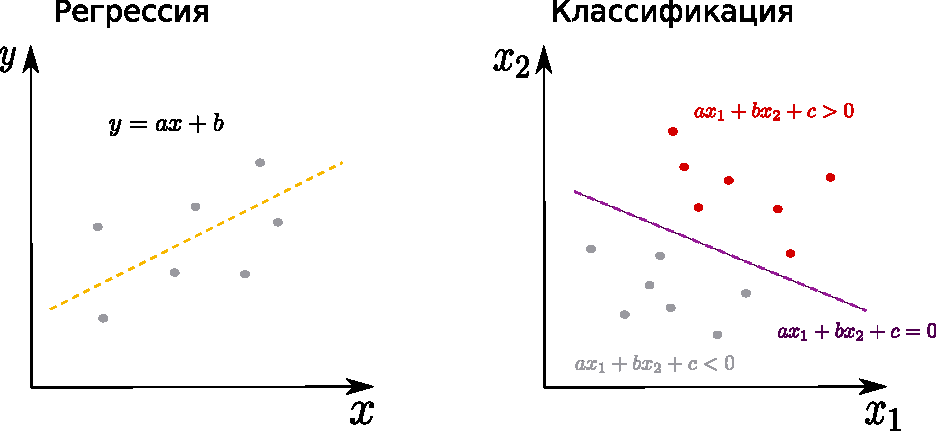
\includegraphics[width=\linewidth]{pictures/linear_models/Class_models.pdf}
	\end{figure}
	
	\subsection{Линейная регрессия и МНК}
	
	Пусть $y = (y_i)_{i=1}^N  \in \mathbb{R}^N, X = (x_i)_{i=1}^N \in \mathbb{R}^{N \times D}$ -- матрица объекты-признаки (i-ая строка -- вектор признаков i-го объекта). Наша линейная функция выглядит следующим образом:
	\begin{equation*}
		f_\omega(x_i) = \langle \omega, x_i \rangle + \omega_0.
	\end{equation*}
	Сделаем так, чтобы наша функция как можно ближе приближала нашу зависимость. Научимся измерять <<плохость>> модели. \textbf{Функция потерь (loss function)} -- функция <<плохости>> модели.
	
	В качестве лосса возьмем: 
	\begin{equation*}
		L(f,X,y) = \|y - f_\omega(X)\|_2^2 = \\
		\|y - f_\omega(X)\|_2^2 = \sum_{i=1}^{N}(y_i - \langle x_i, \omega \rangle)^2
	\end{equation*}
	Минимизируем нашу функцию потерь: $\|y - f_\omega(X)\|_2^2 \rightarrow \mathop{min}_{\omega}$.
	
	\subsection{точный аналитический метод}
	
	Приравняем к нуля градиент по $\omega$ и получим формулу для оптимального вектора весов:
	\begin{equation*}
		\omega_* = \left(X^T X\right)^{-1} X^T y.
	\end{equation*}
	
	Действие получение точного решения вычислительно трудное, а также возможно обратная матрица плохо обусловлена (погрешность вычисления вектора весов зависит от квадрата 	числа обусловленности).
	
	\subsection{приближенный численный метод}
	
	Используем то, что градиент функции в точке направлен в сторону её роста. То есть, мы можем улучшить приближенное оптимальное значение параметра $\omega$, немного сдвинув его в направлении антиградиента:
	\begin{equation*}
		\omega_j \mapsto \omega_j - \alpha \frac{d}{d \omega_j} L,
	\end{equation*}
	где $\alpha$ -- \textbf{темп обучения}. Описанный алгоритм называется \textbf{градиентным спуском}.
	
	Градиент функции потерь:
	\begin{equation*}
		\nabla_w L = 2 X^T \left(X\omega - y\right).
	\end{equation*}
	
	\textbf{Алгоритм градиентного спуска}:
	\begin{lstlisting}
		w = random_normal()
		repeat S times:
		f = X.dot(w)
		err = f - y
		grad = 2 * X.T.dot(err) / n
		w -= alpha * grad
	\end{lstlisting}
	
	Вычислительная сложность градиентного спуска -- $O(NDS)$, где $N$ -- длина выборки, $D$ -- число признаков, $S$ -- число итераций.
	
	Сложность по памяти -- $O(ND)$.
	
	\subsection{Стохастический градиентный спуск}
	
	Возникает идея заменить градиент его оценкой на подвыборке (\textbf{batch, mini-batch}). Используют линейный проход по выборке, при котором на $В$ очередных примерах ($B$ -- размер батча) вычисляется градиент и производится обновление весов модели. Количество шагов задают количеством \textbf{эпох} $E$ -- полным проходом по выборке.
	
	\textbf{Алгоритм}:
	\begin{lstlisting}
		w = normal(0,1)
		repeat E times:
		for i = B, i <= n, i += B:
		X_batch = x[i-B : i]
		Y_batch = y[i-B : i]
		f = X_batch.dot(w)
		err = f - Y_batch
		grad = 2 * X_batch.T.dot(err) / n
		w -= alpha * grad
	\end{lstlisting}
	
	Сложность по времени -- $O(NDE)$.
	
	Сложность по памяти -- $O(BD)$ (всю выборку не надо держать в памяти, достаточно только загружать лишь текущий батч)
	
	\newpage
	
	\begin{figure}[h!]
		\centering
		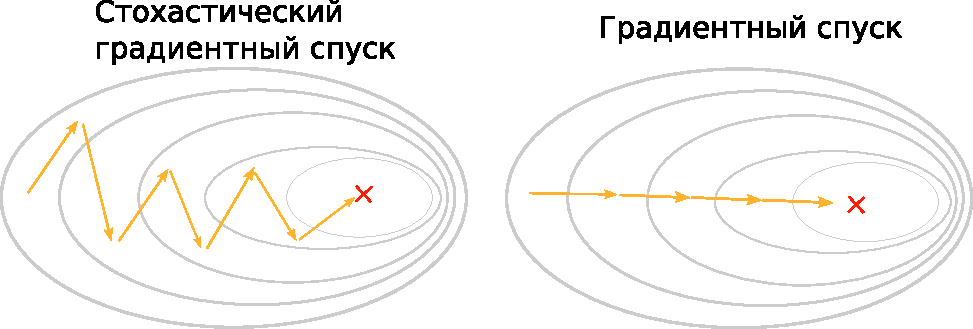
\includegraphics[width=\linewidth]{pictures/linear_models/SGD_GD.pdf}
	\end{figure}
	
	\subsection{Регуляризация}
	
	Бывает так, что признаки могут быть приближенно линейно зависимыми -- \textbf{мультиколлинеарность}. Симметричная матрица, которую впоследствии должны обратить, близка к вырожденной. Некоторые из собственных чисел будут близки к нулю. Из этого будет следовать умножение на $\frac{1}{\lambda_i}$ в нахождении вектора весов, что влечет к появлению больших по модулю чисел.
	
	Чтобы справиться с этим задачу \textbf{регуляризуют} -- добавляют дополнительное ограничение на величину вектора весов. Вместо исходной задачи имеем:
	\begin{equation*}
		\min_\omega L(f,X,y) = \min_w (\|X\omega-y\|^2_2 + \lambda \|\omega\|^k_k),
	\end{equation*}
	где $\lambda \|\omega\|^k_k$ -- \textbf{регуляризационный член}, $\lambda$ -- \textbf{коэффициент регуляризации}.
	
	Отметим, что $\omega_0$ не имеет смысла регуляризировать, т. е. например:
	\begin{equation*}
		\|\omega\|^2_2 = \sum_{j=1}^{D} \omega_j^2
	\end{equation*}
	
	В случае $L^2$-регуляризации, продифференцировав новый лосс, получим <<точное>> решение:
	\begin{equation*}
		\omega = (X^TX + \lambda I)^{-1}X^Ty.
	\end{equation*}
	Градиент функции потерь:
	\begin{equation*}
		\nabla_\omega L(f_\omega, X, y) = 2X^T(X\omega - y) + 2\lambda\omega
	\end{equation*}
	
	\subsection{Разрежение весов в $L^1$-регуляризации}
	
	Существует полезная особенность данной рпегуляризации: её применение приводит к тому, что у признаков, которые не оказывают большого влияния на ответ, вес в результате оптимизации получается равным нулю.
	
	\subsection{Другие лоссы}
	
	\textbf{Mean absolute error}, абсолютная ошибка:
	\begin{equation*}
		MAE(y,\widehat{y}) = \frac{1}{N} \sum_{i=1}^{N}|y_i - \widehat{y_i}|.
	\end{equation*} 
	\textbf{Mean absolute percentage error}, относительная ошибка:
	\begin{equation*}
		MAPE(y,\widehat{y}) = \frac{1}{N} \sum_{i=1}^{N}\left|\frac{\widehat{y_i} - y_i}{y_i}\right|.
	\end{equation*}
	
	\subsection{Линейная классификация}
	
	Рассмотрим классификацию на 2 класса. Обучим линейную модель строить плоскость, которая будет как можно лучше отделять объекты одного класса от другого.
	
	Выборка, для которой возможна плоскость, которая идеально разделит классы, называется \textbf{линейно разделимой}.
	
	Итоговое предсказание вычисляется по формуле:
	\begin{equation*}
		y = sign\langle \omega,x_i \rangle.
	\end{equation*}
	Минимизируем число ошибок предсказателя:
	\begin{equation*}
		\sum_{i}^{} \mathbb{I}[y_i \not= sign\langle \omega,x_i \rangle] \rightarrow \min_\omega
	\end{equation*}
	Домножим обе части на $y_i$ и упростим:
	\begin{equation*}
		\sum_{i}^{} \mathbb{I}[y_i\langle \omega,x_i \rangle < 0] \rightarrow \min_\omega,
	\end{equation*}
	где $M = y_i\langle \omega,x_i \rangle$ -- \textbf{отступ (margin)} классификатора, ошибка -- \textbf{misclassification loss}.
	То есть, имеем функцию:
	\begin{equation*}
		F(M) = \mathbb{I}[M < 0] = 
		\begin{gathered}
			1,\quad M < 0 \\
			0,\quad M \geq 0
		\end{gathered}
	\end{equation*}
	Мажорируем её более гладкой функцией (кусочно-постоянную функцию невозможно оптимизировать градиентными методами). Некоторые из них:
	\begin{itemize}
		\item Перцептрон: $max(0, -M_i)$
		\item Hinge (SVM): $max(0, 1-M_i)$
	\end{itemize}
	
	Лосс перцептрона с $L^2$-регуляризации:
	\begin{equation*}
		L(\omega, x, y) = \lambda \|\omega\|^2_2 + \sum_{i}^{} \max(0,-y_i\langle \omega, x_i \rangle)
	\end{equation*}
	Градиент функции потерь:
	\begin{equation*}
		\nabla_\omega L(\omega, x, y) = 2 \lambda \omega + \sum_{i}^{}
		\begin{gathered}
			0,\quad y_i\langle \omega, x_i \rangle > 0 \\
			- y_i x_i,\quad y_i\langle \omega, x_i \rangle \leq 0
		\end{gathered}
	\end{equation*}
	
	Возникает желание не только найти разделяющую прямую, но и постараться провести её на одинаковом удалении от обоих классов, то есть максимизировать минимальный отступ. Для этого слегка поменяем функцию ошибки на Hinge. Лосс в этом случае:
	\begin{equation*}
		L(\omega, x, y) = \lambda \|\omega\|^2_2 + \sum_{i}^{} \max(0, 1 - y_i\langle \omega, x_i \rangle)
	\end{equation*}
	Градиент:
	\begin{equation*}
		\nabla_\omega L(\omega, x, y) = 2 \lambda \omega + \sum_{i}^{}
		\begin{gathered}
			0,\quad 1 - y_i\langle \omega, x_i \rangle \leq 0 \\
			- y_i x_i,\quad 1 - y_i\langle \omega, x_i \rangle > 0
		\end{gathered}
	\end{equation*}
	
	Ближайшие к плоскости правильно классифицированные объекты называют \textbf{опорные векторы (support vectors)}. Итоговое положение задается такими обучающимися примерами -- такой зовется \textbf{метод опорных векторов (support vector machine)}.
	
	\subsection{Логистическая регрессия}
	
	Появляется желание посмотреть на классификацию, как на задачу предсказания вероятностей. Научим линейную модель предсказывать какой-то объект, связанный с вероятностью, но с диапазоном значений $(-\infty, +\infty)$. Таким объектом является \textbf{logit} или \textbf{log odds}: $\log\left(\frac{p}{1-p}\right)$. Тогда:
	\begin{equation*}
		\langle\omega,x_i\rangle = \log\left(\frac{p}{1 - p}\right)
	\end{equation*}
	\begin{equation*}
		e^{\langle\omega,x_i\rangle}  = \frac{p}{1 - p}
	\end{equation*}
	\begin{equation*}
		p = \frac{1}{1 + e^{-\langle\omega,x_i\rangle}}.
	\end{equation*}
	Данная фукнция называется \textbf{сигмоидой} и обозначается $\sigma(z) = \frac{1}{1 + e^{-z}}$.
	
	Для наилучшей оптимизации $\omega$ применим метод максимума правдоподобия для распределения Бернулли. Оно позволяет нам понять, насколько вероятно получить данные значения таргета $y$ при данных $X$ и весах $\omega$:
	\begin{equation*}
		p\left(y | X,\omega\right) = \prod_i p(y_i | x_i, \omega).
	\end{equation*}
	Для распределения Бернулли:
	\begin{equation*}
		p\left(y | X,\omega\right) = \prod_i p_i^{y_i} (1 - p_i)^{1 - y_i},
	\end{equation*}
	где $p_i$ -- вероятность, посчитанная из ответов модели. Перейдём к логарифмическому правдоподобию и подставим прошлую формулу:
	\begin{multline*}
		l\left(\omega, X, y\right) = \sum_{i}(y_i \log(p_i) + (1 - y_i) \log(1 - p_i)) = \\
		= \sum_{i}(y_i \log(\sigma(\langle \omega, x_i \rangle)) + (1 - y_i) \log(1 - \sigma(\langle\omega,x_i\rangle))) 
	\end{multline*}
	Так как $\sigma(-z) = \frac{1}{1 + e^z} = \frac{e^{-z}}{e^{-z} + 1} = 1 - \sigma(z)$, то:
	\begin{equation*}
		l(\omega, X, y) = \sum_{i}(y_i \log(\sigma(\rangle\omega,x_i\rangle)) + (1 - y_i)\log(\sigma(-\langle\omega,x_i\rangle))).
	\end{equation*}
	
	В максимуме данной отрицательной фукнции находится наше оптимизицанное значение $\omega$. Для минимизации функциЯ лосса выглядит следующим образом:
	\begin{equation*}
		L(\omega, X, y) = -\sum_{i}(y_i \log(\sigma(\rangle\omega,x_i\rangle)) + (1 - y_i)\log(\sigma(-\langle\omega,x_i\rangle))).
	\end{equation*}
	
	Градиент функции:
	\begin{equation*}
		\nabla_\omega L(y, X, \omega) = - \sum_{i} x_i (y_i - \sigma(\langle\omega,x_i\rangle))).
	\end{equation*}
	
	Наше предсказание лежит в пределе от 0 до 1. Находить порог между этими двумя классами
	лучше отдельно, для уже построенной регрессии, минимизируя нужную метрику на отложенной тестовой выборке.
	
	\chapter{Основные алгоритмы}
	
	\section{Backpropagation}
	
	\subsection{Вступление}
	
	Алгоритмически описать данный процесс достаточно просто:
	
	\begin{itemize}
		\item Вычислить функцию потерь $C(w)$
		\item Вычислить градиент функции $C(w)$, учитывая все веса $(w)$ и биасы $(b)$ в нейронной сети
		\item Изменить веса $(w)$ и биасы $(b)$ пропорционально значению их градиента
	\end{itemize}
	
	Намного сложнее разобраться в том, как в действительности вычисляются эти градиенты.
	
	\subsection{Почему вообще нужно задумываться о том, как работает BP?}
	
	\subsection{Простейший пример}
	
	Рассмотрим следующую нейронную сеть:
	
	\begin{figure}[h!]
		\centering
		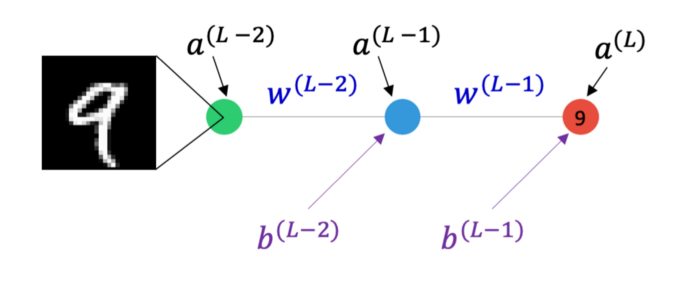
\includegraphics[width=\linewidth]{pictures/backpropagation/1-1-1_network.png}
		\caption{простейшая нейронная сеть}
		\label{simplest_nn}
	\end{figure}
	
	На рисунке \ref{simplest_nn} изображена простейшая нейронная сеть, где зелёный, синий и красный нейрон отвечают за входной, скрытый и выходной нейрон (слой, если говорить в терминах более крупных нейронных сетей) соответственно. Обозначим функцию активации последнего нейрона как $a^{(L)}$, функцию активации предпоследнего слоя как $a^{(L-1)}$, а функцию активации первого слоя как $a^{(L-2)}$, где $L$ - количество слоёв в нашей нейронной сети (в нашем случае $L=3$). Аналогично определим веса и биасы между слоем $L-1$ и $L$ как $w^{(L-1)}$ и $b^{(L-1)}$.
	
	Представим, что наша картинка цифры $9$ состоит из одного пикселя (понятно, что это не возможно; сделаем это для упрощения вычислений). Теперь, пусть после того, как этот один пиксель прошёл через все три слоя нашей простейшей нейронной сети (стадия прямого распространения), на выходе мы получили число 0.68 (так как мы решаем задачу классификации, то выходные значения должны находиться в диапазоне от 0 до 1, что можно интерпретировать как вероятность; для этого можно в качестве функции активации последнего слоя (в нашем случае нейрона) использовать функцию Softmax (добавить сюда потом ссылку)). Но наше желаемое выходное значение --- это 1 (т.е. мы хотим (после завершения обучения), чтобы наша сеть была уверена на 100\%, что данная картинка (в нашем случае один пиксель) --- это число 9). Теперь, пусть мы будем использовать средне квадратичную ошибку в качестве функции потерь. Т.е. мы получаем, что потеря $C$ для одного тренировочного образца (т.е цифры 9) равняется $(0.68-1)^2$
	
	\subsection{Слой $L-1$}
	
	Рассчитаем градиент нашей функуии потерь $C$ учитывая вес, соединяющий нейроны в слое $L$ со слоем $L-1$. Чтобы посмотреть, как бы мы это сделали, развернём последний слой нашей простейшей нейронной сети.
	
	\begin{figure}[h!]
		\centering
		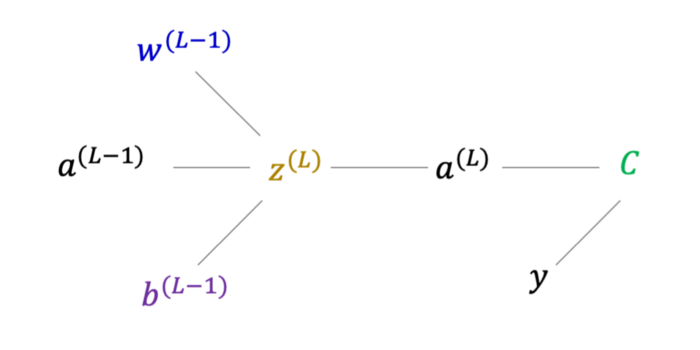
\includegraphics[width=\linewidth]{pictures/backpropagation/last_layer.png}
		\caption{Последний слой}
		\label{last_layer}
	\end{figure}
	
	Фигура \ref{last_layer} показывает, как каждый параметер последних двух слоёв влияет на потерю $C$. Чтобы получить взвешенную сумму $z^{(L)}$ для последнего слоя, мы умножаем активацию слоя (т.е. выход предпоследнего слоя, к которому была применена соответствующая функция активации для даного слоя) $L-1$ на вес $w^{(L-1)}$, соединяющий два слоя, а затем мы прибавляем биас $b^{(L-1)}$. И наконец, мы пропускаем взвешенную сумму через нелинейную функцию (функцию активации) $\sigma(z^{(L)})$, чтобы посчитать $a^{(L)}$.
	
	\begin{figure}[h!]
		\centering
		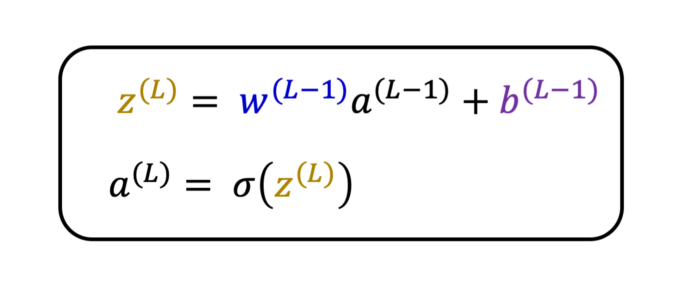
\includegraphics[width=\linewidth]{pictures/backpropagation/sigma.png}
		\caption{Функция активации}
		\label{weighted_sum}
	\end{figure}
	
	Теперь мы хотим посмотреть, как сильно изменится $C$, если мы изменим $w^{(L-1)}$. Т.е. мы хотим посчитать $\dfrac{\partial C}{\partial w^{(L-1)}}$.
	
	\begin{figure}[h!]
		\centering
		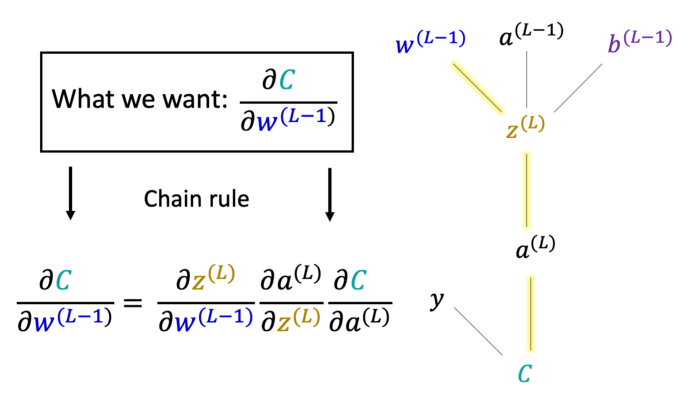
\includegraphics[width=\linewidth]{pictures/backpropagation/chain_rule.png}
		\caption{Дифференцирование}
		\label{derivative_1}
	\end{figure}
	
	Из картинки \ref{derivative_1} можно понять, как вес $w^{(L-1)}$ влияет на $C$. Сначала вес $w^{(L-1)}$ даёт вклад во взвешенную сумму $z^{(L)}$, которая используется для того, чтобы посчитать потерю $C$. Найдём частную производную $\dfrac{\partial C}{\partial w^{(L-1)}}$ явно.
	
	\begin{figure}[h!]
		\centering
		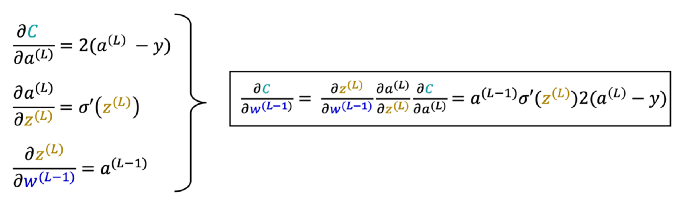
\includegraphics[width=\linewidth]{pictures/backpropagation/derivative_itself.png}
		\caption{Находим частную производную явно}
		\label{derivative_itself_weight}
	\end{figure}
	
	То, как получены последние два выражения в левой части - очевидно. Рассмотрим первое. Так как для подсчёта потери мы используем средне квадратичную ошибку (MSE, которая считается как $(a^{(L)}-y)^2$), то если взять от этого производную по $\partial a^{(L)}$, то мы как раз получим $2(a^{(L)}-y)$.
	
	Заметим, что мы не нашли производную от нашей функции активации (которую мы обозначили как $\sigma$) явно. Если бы мы использовали Sigmoid в качестве нашей функции активации:
	
	\[\dfrac{1}{1+e^{-z}}\]
	
	Тогда её производная равнялась бы:
	
	\[\dfrac{e^{-z}}{(1+e^{-z})^2}\]
	
	\textbf{Замечание:} вот почему важно использовать в качестве функций активации всюду дифференцируемые функции, в противном случае мы не сможем рассчитать наши градиенты, однако функцию ReLu всё же можно использовать (добавить потом сюда ссылку).
	
	Также мы хотим знать, как изменится значение нашей функции потерь, если мы изменим биас $b^{(L-1)}$.
	
	\begin{figure}[h!]
		\centering
		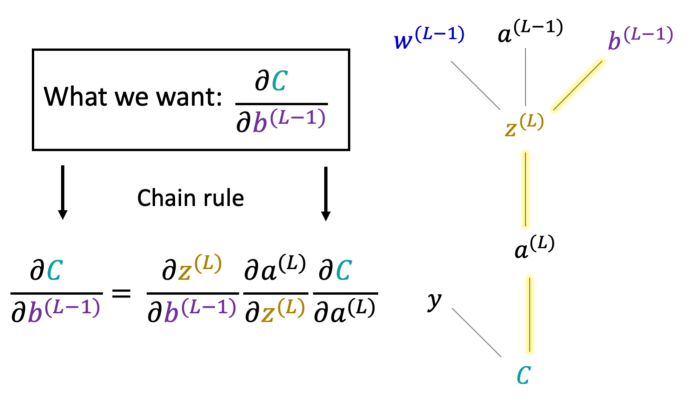
\includegraphics[width=\linewidth]{pictures/backpropagation/bias.png}
		\caption{Считаем производную для биаса}
		\label{derivative_bias}
	\end{figure}
	
	Как можно заметить, поменялся только первый множитель. Аналогично, найдём явную производную.
	
	\begin{figure}[h!]
		\centering
		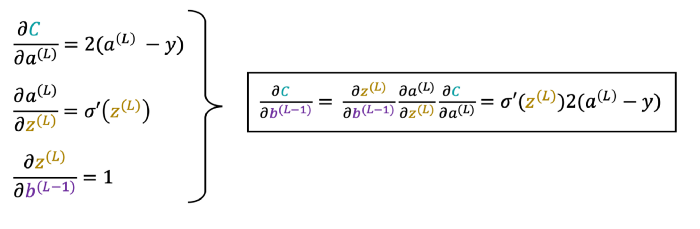
\includegraphics[width=\linewidth]{pictures/backpropagation/derivative_itself_bias.png}
		\caption{Считаем производную для биаса}
		\label{derivative_itself_bias}
	\end{figure}
	
	Отлично, теперь нейронная сеть может использовать полученные выражения для обновления весов и биасов по следующему принципу.
	
	\begin{figure}[h!]
		\centering
		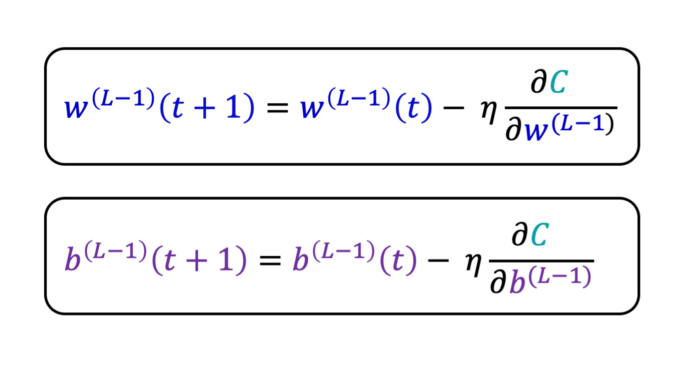
\includegraphics[width=\linewidth]{pictures/backpropagation/updating.png}
		\caption{Обновление весов}
		\label{updating}
	\end{figure}
	
	На картинке \ref{updating} $\eta$ --- это learning rate.
	
	Несмотря на то, что нейронная сеть не имеет прямого контроля над $a^{(L-1)}$, скоро будет показано, что что нам будет это нужно, чтобы дальше двигаться по сети и обновлять параметры, поэтому проделаем предыдущие шаги, только для $a^{(L-1)}$.
	
	Получаем:
	
	\begin{figure}[h!]
		\centering
		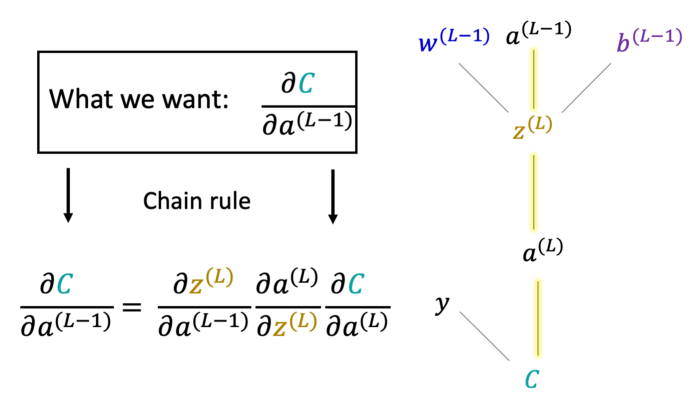
\includegraphics[width=\linewidth]{pictures/backpropagation/last_activation.png}
		\caption{Считаем градиент относительно функции активации предпоследнего слоя}
		\label{last_activation}
	\end{figure}
	
	Находим производную явно:
	
	\begin{figure}[h!]
		\centering
		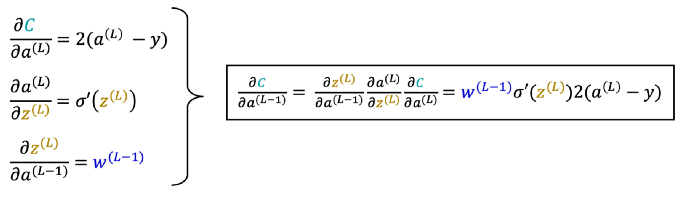
\includegraphics[width=\linewidth]{pictures/backpropagation/last_activation_itself.png}
		\caption{Находим производную явно}
		\label{last_activation_itself}
	\end{figure}
	
	\subsection{Слой $L-2$}
	
	Теперь давайте посмотрим, как будет меняться значение функции потерь $C$, если изменять параметры в слое $L-2$. Как и раньше, нарисуем граф, чтобы наглядо продемонстрировать, как $w^{(L-2)}$ и $b^{(L-2)}$ косвенно влияют на значение потери $C$.
	
	\begin{figure}[h!]
		\centering
		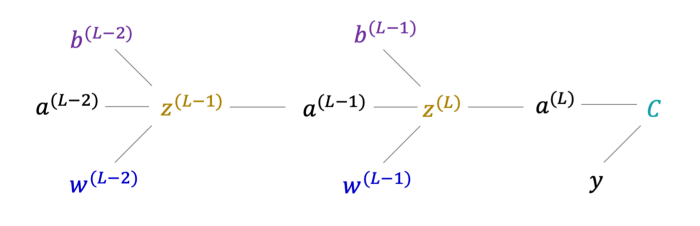
\includegraphics[width=\linewidth]{pictures/backpropagation/first_layer.png}
		\caption{Слои $L-1$ и $L-2$}
		\label{first_layer}
	\end{figure}
	
	Аналогично, используя цепное правило, посмотрим, как изменение веса $w^{(L-2)}$ влияет на значение функции потерь $C$.
	
	\begin{figure}[h!]
		\centering
		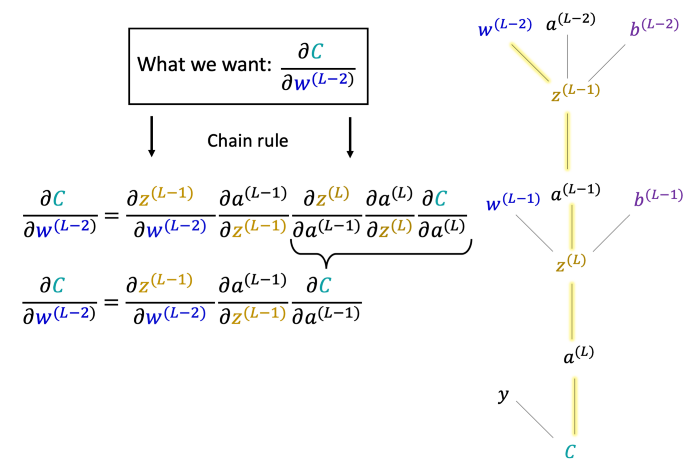
\includegraphics[width=\linewidth]{pictures/backpropagation/first_layer_weight.png}
		\caption{Частная производная для веса первого слоя}
		\label{first_layer_weight}
	\end{figure}
	
	Теперь найдём производную явно:
	
	\begin{figure}[h!]
		\centering
		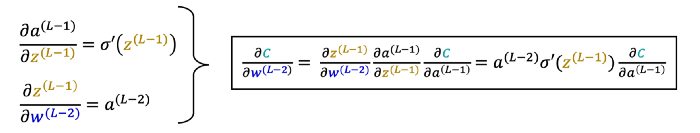
\includegraphics[width=\linewidth]{pictures/backpropagation/first_layer_itself.png}
		\caption{Производная в явном виде}
		\label{first_layer_itself}
	\end{figure}
	
	Аналогичным образом можно посчитать градиенты для всех весов и биасов. Этот алгоритм называется \textbf{обратным распространением ошибки}.
	
	
	
	
	
	
	
	
	
	
	
	
	
	
	
	
	
	
	
	
	
	
\end{document}